\documentclass[11pt]{article}
\usepackage{mathblatt}
% gesetzt von werkzeuge/setzer.py (Sorte selbst) aus dem Lernweg XKT
% und den Bankzeilen; Muster bau/proben/2026-10-09/hypotenuse-muster.
\usepackage{enumitem}
\usepackage{adjustbox,varwidth}
\newgeometry{a4paper,margin=18mm,top=15mm,bottom=20mm,footskip=9mm}
\pagestyle{fancy}\fancyhf{}\renewcommand{\headrulewidth}{0pt}
\fancyfoot[L]{\footnotesize\color{mbgrau}XKT \textperiodcentered{} Ohne Zurücklegen}
\fancyfoot[R]{\footnotesize\color{mbgrau}\thepage}
\setlength{\parskip}{3pt}
\renewcommand{\kreuz}[1]{\mbox{$\square$\ #1}\quad}
\newcommand{\kreuzl}[1]{\par\hangindent1.4em\hangafter1\noindent$\square$\ #1}
\newcommand{\aufg}[3]{\par\noindent\makebox[0pt][r]{#3}\begin{minipage}[t]{\linewidth}#1\end{minipage}\par}
\newcommand{\aufgg}[4]{\par\noindent\makebox[0pt][r]{#4}\begin{minipage}[t]{0.6\linewidth}\vspace{0pt}#1\end{minipage}\hfill
  \begin{minipage}[t]{0.37\linewidth}\vspace{0pt}\centering #2\end{minipage}\par}
\newcommand{\nr}[1]{\makebox[7mm][l]{\textbf{#1}}}
\newcommand{\lsg}[3]{\par\noindent\begin{minipage}[t]{9mm}\textbf{#1}\end{minipage}%
  \begin{minipage}[t]{52mm}\raggedright\bfseries\boldmath #2\end{minipage}\hspace{3mm}%
  \begin{minipage}[t]{\dimexpr\linewidth-64mm\relax}\raggedright\small #3\end{minipage}\par\vspace{4pt}}
\newlength{\kr}
\makeatletter
\newcommand{\karomerk}[2]{\protected@write\@auxout{}{\string\karoseite{#1}{#2}{\thepage}}}
\newcommand{\karoseite}[3]{\expandafter\xdef\csname karo@#1@#2\endcsname{#3}}
\newcommand{\karohinweis}[3]{\karomerk{h}{#1}\ifcsname karo@k@#1\endcsname
  \ifnum\csname karo@k@#1\endcsname=0\csname karo@h@#1\endcsname\relax#2\else#3\fi
  \else#3\fi}
\makeatother
\begin{document}

\noindent{\LARGE\bfseries Ohne Zurücklegen}\par\smallskip
\noindent{\small\color{mbgrau}Selbstlernheft Klasse 9 \textperiodcentered{} mit Lösungsheft \textperiodcentered{} Kennung XKT}\par\medskip
\noindent\textbf{So nutzt du das Heft:} Lies im Abschnitt das Beispiel. Rechne dann die Aufgaben der Reihe nach und vergleiche jede sofort mit dem Lösungsheft. Kreuze „kann ich“ an, wenn du die letzte Aufgabe (\emph{Ziel}) allein schaffst.\par
\noindent Mehr Aufgaben zu einem Abschnitt: Kennung deinem Nachhilfelehrer schicken (z.\,B. „XKT mehr B“).\par\medskip
{\arrayrulecolor{mbgrau}\renewcommand{\arraystretch}{1.3}
\noindent\begin{tabular}{|>{\bfseries}p{10mm}|p{112mm}|>{\raggedleft\arraybackslash}p{10mm}|>{\centering\arraybackslash}p{14mm}|}\hline
\rowcolor{black!8} & \textbf{Abschnitt} & \textbf{Seite} & \textbf{kann ich}\\\hline
A & Zweimal ziehen: eins weniger & \pageref{s:A} & $\square$\\\hline
B & Mehrere Pfade, zweite Person & \pageref{s:B} & $\square$\\\hline
C & Drei Züge & \pageref{s:C} & $\square$\\\hline
D & Mit oder ohne Zurücklegen? & \pageref{s:D} & $\square$\\\hline
T & Probetest & \pageref{s:T} & $\square$\\\hline
\end{tabular}}\par\bigskip

\begin{tcolorbox}[colback=mbkasten,colframe=mbgrau,boxrule=0.5pt,arc=1mm,left=3mm,right=3mm,top=2mm,bottom=2mm,title={\bfseries Formel auf einen Blick},coltitle=black,colbacktitle=black!10]
{\Large Pfad: mal \qquad mehrere Pfade: plus}\par\medskip
\textbf{So gehst du vor}\par
\nr{1}lesen, ob das Gezogene zurückkommt\par
\nr{2}Baum zeichnen, nach jedem Zug Nenner und Zähler anpassen\par
\nr{3}die Pfade zum Ereignis suchen\par
\nr{4}je Pfad multiplizieren, die Pfade addieren\par
\medskip
\end{tcolorbox}
\clearpage\label{s:A}\noindent\colorbox{black!12}{\makebox[10mm]{\Large\bfseries\strut A}}\hspace{3mm}{\Large\bfseries Zweimal ziehen: eins weniger}\par\smallskip
\noindent Ohne Zurücklegen fehlt beim 2. Zug das erste Stück: Der Nenner ist um 1 kleiner, bei der gezogenen Sorte auch der Zähler. Darum hat die 2. Stufe nach jedem Ast der 1. Stufe andere Zahlen.\par\medskip
\noindent\textbf{Formel}\par\nopagebreak\noindent\hspace*{4mm}\begin{minipage}{\dimexpr\linewidth-4mm\relax}$P(\text{zweimal Rot}) = \dfrac{\text{rote}}{\text{alle}} \cdot \dfrac{\text{rote} - 1}{\text{alle} - 1}$\end{minipage}\par\medskip
\noindent\textbf{Beispiel}\quad In einem Beutel liegen 3 rote (R) und 2 blaue (B) Kugeln. Zwei Kugeln werden nacheinander gezogen, ohne Zurücklegen. Wie groß ist die Wahrscheinlichkeit für zweimal Rot?\par\smallskip
\noindent\begin{minipage}[t]{0.6\linewidth}\vspace{0pt}\par\noindent\hangindent6mm\hangafter1\makebox[6mm][l]{\textbf{1}}1. Zug: 5 Kugeln, davon 3 rote: R $\frac{3}{5}$, B $\frac{2}{5}$.\par\smallskip\par\noindent\hangindent6mm\hangafter1\makebox[6mm][l]{\textbf{2}}Nach Rot liegen noch 4 Kugeln da, nur noch 2 rote: R $\frac{2}{4}$, B $\frac{2}{4}$. Nach Blau: R $\frac{3}{4}$, B $\frac{1}{4}$.\par\smallskip\par\noindent\hangindent6mm\hangafter1\makebox[6mm][l]{\textbf{3}}Pfad R – R nachfahren und multiplizieren: $\frac{3}{5} \cdot \frac{2}{4} = \frac{6}{20} = \frac{3}{10}$.\par\smallskip\par\noindent\hangindent6mm\hangafter1\makebox[6mm][l]{\textbf{4}}Die Wahrscheinlichkeit für zweimal Rot ist $\frac{3}{10}$.\par\smallskip\end{minipage}\hfill
\begin{minipage}[t]{0.37\linewidth}\vspace{0pt}\centering 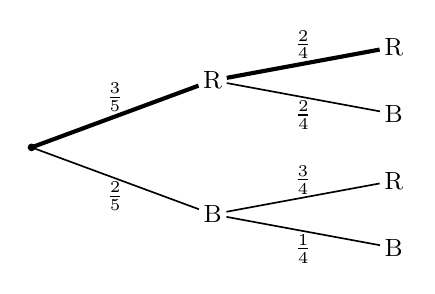
\begin{tikzpicture}[ak/.style={font=\small,inner sep=1.5pt,fill=white},wk/.style={font=\footnotesize,inner sep=1pt}]\fill (0,0) circle (1.4pt);\coordinate (s) at (0,0);\node[ak] (nR) at (2.30,0.850) {R};\node[ak] (nRR) at (4.60,1.275) {R};\node[ak] (nRB) at (4.60,0.425) {B};\node[ak] (nB) at (2.30,-0.850) {B};\node[ak] (nBR) at (4.60,-0.425) {R};\node[ak] (nBB) at (4.60,-1.275) {B};\draw[line width=1.5pt] (s) -- (nR) node[wk,above,pos=0.5] {$\frac{3}{5}$};\draw[line width=1.5pt] (nR) -- (nRR) node[wk,above,pos=0.5] {$\frac{2}{4}$};\draw[line width=0.6pt] (nR) -- (nRB) node[wk,below,pos=0.5] {$\frac{2}{4}$};\draw[line width=0.6pt] (s) -- (nB) node[wk,below,pos=0.5] {$\frac{2}{5}$};\draw[line width=0.6pt] (nB) -- (nBR) node[wk,above,pos=0.5] {$\frac{3}{4}$};\draw[line width=0.6pt] (nB) -- (nBB) node[wk,below,pos=0.5] {$\frac{1}{4}$};\end{tikzpicture}\end{minipage}\par\medskip
\noindent\textbf{Aufgaben}\hspace{1em}{\small\color{mbgrau}\karohinweis{A}{Rechne unten im Karo.}{Rechne auf einem extra Blatt.} Vergleiche jede Aufgabe gleich mit dem Lösungsheft.}\par\smallskip
\aufg{\hangindent7mm\hangafter1\nr{1.}In einer Dose liegen 7 Kekse, 3 davon mit Schokolade. Lea isst einen Schokokeks. Wie viele Kekse liegen noch in der Dose, wie viele davon mit Schokolade? Wie groß ist jetzt die Wahrscheinlichkeit, einen Schokokeks zu greifen?}{}{}
\medskip
\aufgg{\hangindent7mm\hangafter1\nr{2.}In einem Beutel liegen 2 gelbe (G) und 4 weiße (W) Kugeln. Zwei werden ohne Zurücklegen gezogen. Ergänze im Baum die Äste der 2. Stufe. Wie groß ist die Wahrscheinlichkeit für zuerst Gelb, dann Weiß?}{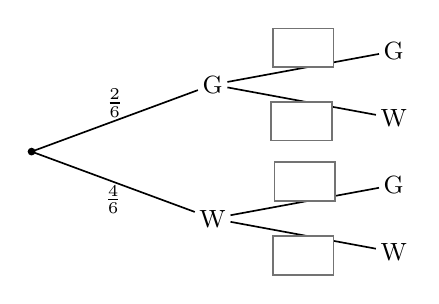
\begin{tikzpicture}[ak/.style={font=\small,inner sep=1.5pt,fill=white},wk/.style={font=\footnotesize,inner sep=1pt}]\fill (0,0) circle (1.4pt);\coordinate (s) at (0,0);\node[ak] (nG) at (2.30,0.850) {G};\node[ak] (nGG) at (4.60,1.275) {G};\node[ak] (nGW) at (4.60,0.425) {W};\node[ak] (nW) at (2.30,-0.850) {W};\node[ak] (nWG) at (4.60,-0.425) {G};\node[ak] (nWW) at (4.60,-1.275) {W};\draw[line width=0.6pt] (s) -- (nG) node[wk,above,pos=0.5] {$\frac{2}{6}$};\draw[line width=0.6pt] (nG) -- (nGG) node[wk,above,draw=black!55,fill=white,pos=0.5] {\rule{0pt}{4.2mm}\rule{7mm}{0pt}};\draw[line width=0.6pt] (nG) -- (nGW) node[wk,below,draw=black!55,fill=white,pos=0.5] {\rule{0pt}{4.2mm}\rule{7mm}{0pt}};\draw[line width=0.6pt] (s) -- (nW) node[wk,below,pos=0.5] {$\frac{4}{6}$};\draw[line width=0.6pt] (nW) -- (nWG) node[wk,above,draw=black!55,fill=white,pos=0.5] {\rule{0pt}{4.2mm}\rule{7mm}{0pt}};\draw[line width=0.6pt] (nW) -- (nWW) node[wk,below,draw=black!55,fill=white,pos=0.5] {\rule{0pt}{4.2mm}\rule{7mm}{0pt}};\end{tikzpicture}}{}{}
\medskip
\aufg{\hangindent7mm\hangafter1\nr{3.}Von 10 Losen sind 3 Gewinne. Tom zieht nacheinander zwei Lose und behält sie. Wie groß ist die Wahrscheinlichkeit, dass beide gewinnen?}{}{}
\medskip
\aufg{\hangindent7mm\hangafter1\nr{4.}Lisa darf aus einem von zwei Beuteln zwei Kugeln ziehen, ohne Zurücklegen. Bei zweimal Rot gewinnt sie. Im Beutel 1 liegen 3 rote und 1 blaue Kugel, im Beutel 2 liegen 6 rote und 2 blaue. Lisa meint: „Der Anteil Rot ist gleich, also ist es egal.“ Hat sie recht? Begründe mit den Wahrscheinlichkeiten.}{}{{\scriptsize\color{mbgrau}Ziel\hspace{2mm}}}
\medskip
\par\vspace{3mm}\setlength{\kr}{\dimexpr\pagegoal-\pagetotal-10mm\relax}%
\ifdim\kr>12mm\karomerk{k}{A}\noindent{\scriptsize\color{mbgrau}Platz zum Rechnen}\par\nointerlineskip\vspace{1mm}\noindent
\begin{tikzpicture}\clip (0,0) rectangle ({\linewidth-0.5mm},\kr);\draw[black!16,line width=0.3pt,step=5mm] (0,0) grid (\linewidth,\kr);\end{tikzpicture}\fi\par
\clearpage\label{s:B}\noindent\colorbox{black!12}{\makebox[10mm]{\Large\bfseries\strut B}}\hspace{3mm}{\Large\bfseries Mehrere Pfade, zweite Person}\par\smallskip
\noindent Gehören mehrere Pfade zum Ereignis, rechnest du jeden Pfad mit seinen eigenen Ästen und addierst. Fragt man, was die zweite Person zieht, gehört der Zug der ersten mit in den Pfad.\par\medskip
\noindent\textbf{Formel}\par\nopagebreak\noindent\hspace*{4mm}\begin{minipage}{\dimexpr\linewidth-4mm\relax}$P(\text{Ereignis}) = P(\text{Pfad 1}) + P(\text{Pfad 2}) + \ldots$\end{minipage}\par\medskip
\noindent\textbf{Beispiel}\quad In einem Beutel liegen 3 rote (R) und 2 blaue (B) Kugeln. Zwei werden ohne Zurücklegen gezogen. Wie groß ist die Wahrscheinlichkeit, dass beide dieselbe Farbe haben?\par\smallskip
\noindent\begin{minipage}[t]{0.6\linewidth}\vspace{0pt}\par\noindent\hangindent6mm\hangafter1\makebox[6mm][l]{\textbf{1}}Dieselbe Farbe: die Pfade R – R und B – B.\par\smallskip\par\noindent\hangindent6mm\hangafter1\makebox[6mm][l]{\textbf{2}}R – R: $\frac{3}{5} \cdot \frac{2}{4} = \frac{6}{20}$. B – B: $\frac{2}{5} \cdot \frac{1}{4} = \frac{2}{20}$.\par\smallskip\par\noindent\hangindent6mm\hangafter1\makebox[6mm][l]{\textbf{3}}Addieren: $\frac{6}{20} + \frac{2}{20} = \frac{8}{20} = \frac{2}{5}$.\par\smallskip\par\noindent\hangindent6mm\hangafter1\makebox[6mm][l]{\textbf{4}}Die Wahrscheinlichkeit für dieselbe Farbe ist $\frac{2}{5}$.\par\smallskip\end{minipage}\hfill
\begin{minipage}[t]{0.37\linewidth}\vspace{0pt}\centering 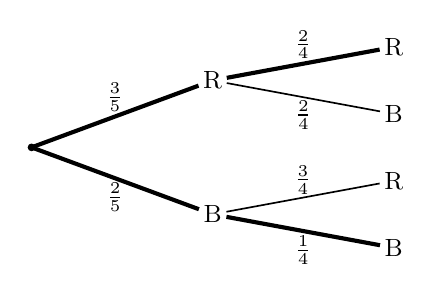
\begin{tikzpicture}[ak/.style={font=\small,inner sep=1.5pt,fill=white},wk/.style={font=\footnotesize,inner sep=1pt}]\fill (0,0) circle (1.4pt);\coordinate (s) at (0,0);\node[ak] (nR) at (2.30,0.850) {R};\node[ak] (nRR) at (4.60,1.275) {R};\node[ak] (nRB) at (4.60,0.425) {B};\node[ak] (nB) at (2.30,-0.850) {B};\node[ak] (nBR) at (4.60,-0.425) {R};\node[ak] (nBB) at (4.60,-1.275) {B};\draw[line width=1.5pt] (s) -- (nR) node[wk,above,pos=0.5] {$\frac{3}{5}$};\draw[line width=1.5pt] (nR) -- (nRR) node[wk,above,pos=0.5] {$\frac{2}{4}$};\draw[line width=0.6pt] (nR) -- (nRB) node[wk,below,pos=0.5] {$\frac{2}{4}$};\draw[line width=1.5pt] (s) -- (nB) node[wk,below,pos=0.5] {$\frac{2}{5}$};\draw[line width=0.6pt] (nB) -- (nBR) node[wk,above,pos=0.5] {$\frac{3}{4}$};\draw[line width=1.5pt] (nB) -- (nBB) node[wk,below,pos=0.5] {$\frac{1}{4}$};\end{tikzpicture}\end{minipage}\par\medskip
\noindent\textbf{Aufgaben}\hspace{1em}{\small\color{mbgrau}\karohinweis{B}{Rechne unten im Karo.}{Rechne auf einem extra Blatt.} Vergleiche jede Aufgabe gleich mit dem Lösungsheft.}\par\smallskip
\aufgg{\hangindent7mm\hangafter1\nr{1.}In Oles Mäppchen liegen 4 blaue (B) und 3 schwarze (S) Stifte. Er nimmt blind zwei heraus. Der Baum ist fertig. a) Wie groß ist die Wahrscheinlichkeit für zwei verschiedene Farben? b) Zu welchem Ereignis gehört die Rechnung $\frac{3}{7} \cdot \frac{2}{6}$?}{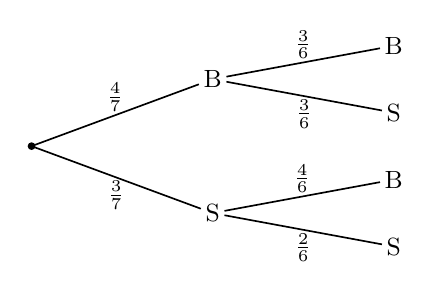
\begin{tikzpicture}[ak/.style={font=\small,inner sep=1.5pt,fill=white},wk/.style={font=\footnotesize,inner sep=1pt}]\fill (0,0) circle (1.4pt);\coordinate (s) at (0,0);\node[ak] (nB) at (2.30,0.850) {B};\node[ak] (nBB) at (4.60,1.275) {B};\node[ak] (nBS) at (4.60,0.425) {S};\node[ak] (nS) at (2.30,-0.850) {S};\node[ak] (nSB) at (4.60,-0.425) {B};\node[ak] (nSS) at (4.60,-1.275) {S};\draw[line width=0.6pt] (s) -- (nB) node[wk,above,pos=0.5] {$\frac{4}{7}$};\draw[line width=0.6pt] (nB) -- (nBB) node[wk,above,pos=0.5] {$\frac{3}{6}$};\draw[line width=0.6pt] (nB) -- (nBS) node[wk,below,pos=0.5] {$\frac{3}{6}$};\draw[line width=0.6pt] (s) -- (nS) node[wk,below,pos=0.5] {$\frac{3}{7}$};\draw[line width=0.6pt] (nS) -- (nSB) node[wk,above,pos=0.5] {$\frac{4}{6}$};\draw[line width=0.6pt] (nS) -- (nSS) node[wk,below,pos=0.5] {$\frac{2}{6}$};\end{tikzpicture}}{}{}
\medskip
\aufg{\hangindent7mm\hangafter1\nr{2.}In Tims Schublade liegen 6 schwarze und 4 weiße Socken. Im Dunkeln nimmt er zwei heraus. Wie groß ist die Wahrscheinlichkeit, dass beide dieselbe Farbe haben? Schreib zuerst die passenden Pfade auf.}{}{}
\medskip
\aufg{\hangindent7mm\hangafter1\nr{3.}In einem Hut liegen 6 Zettel, auf einem steht „Joker“. Erst zieht Ali einen Zettel und behält ihn, dann zieht Bea. Wie groß ist die Wahrscheinlichkeit, dass Bea den Joker zieht?}{}{}
\medskip
\aufg{\hangindent7mm\hangafter1\nr{4.}In einer Box liegen 10 Lose, 2 davon sind Gewinne. Jonas zieht zuerst ein Los und behält es, dann zieht Emma. Emma sagt: „Als Zweite habe ich eine schlechtere Chance auf einen Gewinn.“ Hat sie recht? Vergleiche die Wahrscheinlichkeiten.}{}{{\scriptsize\color{mbgrau}Ziel\hspace{2mm}}}
\medskip
\par\vspace{3mm}\setlength{\kr}{\dimexpr\pagegoal-\pagetotal-10mm\relax}%
\ifdim\kr>12mm\karomerk{k}{B}\noindent{\scriptsize\color{mbgrau}Platz zum Rechnen}\par\nointerlineskip\vspace{1mm}\noindent
\begin{tikzpicture}\clip (0,0) rectangle ({\linewidth-0.5mm},\kr);\draw[black!16,line width=0.3pt,step=5mm] (0,0) grid (\linewidth,\kr);\end{tikzpicture}\fi\par
\clearpage\label{s:C}\noindent\colorbox{black!12}{\makebox[10mm]{\Large\bfseries\strut C}}\hspace{3mm}{\Large\bfseries Drei Züge}\par\smallskip
\noindent Bei drei Zügen wird der Nenner zweimal kleiner. Pfade mit denselben Sorten in anderer Reihenfolge haben dieselbe Wahrscheinlichkeit. Ist eine Sorte aufgebraucht, hat der Punkt nur noch einen Ast.\par\medskip
\noindent\textbf{Formel}\par\nopagebreak\noindent\hspace*{4mm}\begin{minipage}{\dimexpr\linewidth-4mm\relax}$P(\text{dreimal Rot}) = \dfrac{\text{rote}}{\text{alle}} \cdot \dfrac{\text{rote} - 1}{\text{alle} - 1} \cdot \dfrac{\text{rote} - 2}{\text{alle} - 2}$ \qquad $P(\text{mindestens einmal}) = 1 - P(\text{keinmal})$\end{minipage}\par\medskip
\noindent\textbf{Beispiel}\quad In einem Beutel liegen 3 rote (R) und 2 blaue (B) Kugeln. Drei werden ohne Zurücklegen gezogen. Wie groß ist die Wahrscheinlichkeit für genau eine blaue Kugel?\par\smallskip
\noindent\begin{minipage}[t]{0.6\linewidth}\vspace{0pt}\par\noindent\hangindent6mm\hangafter1\makebox[6mm][l]{\textbf{1}}Nach jedem Zug ist eine Kugel weniger da: Nenner 5, 4, 3. Nach zwei blauen gibt es nur noch rote (ein Ast, $\frac{3}{3}$).\par\smallskip\par\noindent\hangindent6mm\hangafter1\makebox[6mm][l]{\textbf{2}}Genau eine blaue: R – R – B, R – B – R, B – R – R.\par\smallskip\par\noindent\hangindent6mm\hangafter1\makebox[6mm][l]{\textbf{3}}Jeder dieser Pfade: $\frac{3}{5} \cdot \frac{2}{4} \cdot \frac{2}{3} = \frac{12}{60}$ – nur die Reihenfolge der Zähler ist anders.\par\smallskip\par\noindent\hangindent6mm\hangafter1\makebox[6mm][l]{\textbf{4}}Drei Pfade addieren: $3 \cdot \frac{12}{60} = \frac{36}{60} = \frac{3}{5}$.\par\smallskip\par\noindent\hangindent6mm\hangafter1\makebox[6mm][l]{\textbf{5}}Mindestens eine blaue geht über das Gegenteil, dreimal Rot: $1 - P(\text{R – R – R}) = 1 - \frac{3}{5} \cdot \frac{2}{4} \cdot \frac{1}{3} = 1 - \frac{6}{60} = \frac{9}{10}$.\par\smallskip\end{minipage}\hfill
\begin{minipage}[t]{0.37\linewidth}\vspace{0pt}\centering 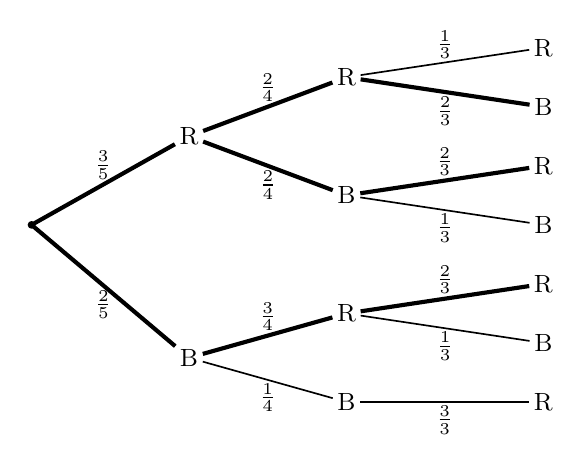
\begin{tikzpicture}[ak/.style={font=\small,inner sep=1.5pt,fill=white},wk/.style={font=\footnotesize,inner sep=1pt}]\fill (0,0) circle (1.4pt);\coordinate (s) at (0,0);\node[ak] (nR) at (2.00,1.125) {R};\node[ak] (nRR) at (4.00,1.875) {R};\node[ak] (nRRR) at (6.50,2.250) {R};\node[ak] (nRRB) at (6.50,1.500) {B};\node[ak] (nRB) at (4.00,0.375) {B};\node[ak] (nRBR) at (6.50,0.750) {R};\node[ak] (nRBB) at (6.50,0.000) {B};\node[ak] (nB) at (2.00,-1.688) {B};\node[ak] (nBR) at (4.00,-1.125) {R};\node[ak] (nBRR) at (6.50,-0.750) {R};\node[ak] (nBRB) at (6.50,-1.500) {B};\node[ak] (nBB) at (4.00,-2.250) {B};\node[ak] (nBBR) at (6.50,-2.250) {R};\draw[line width=1.5pt] (s) -- (nR) node[wk,above,pos=0.5] {$\frac{3}{5}$};\draw[line width=1.5pt] (nR) -- (nRR) node[wk,above,pos=0.5] {$\frac{2}{4}$};\draw[line width=0.6pt] (nRR) -- (nRRR) node[wk,above,pos=0.5] {$\frac{1}{3}$};\draw[line width=1.5pt] (nRR) -- (nRRB) node[wk,below,pos=0.5] {$\frac{2}{3}$};\draw[line width=1.5pt] (nR) -- (nRB) node[wk,below,pos=0.5] {$\frac{2}{4}$};\draw[line width=1.5pt] (nRB) -- (nRBR) node[wk,above,pos=0.5] {$\frac{2}{3}$};\draw[line width=0.6pt] (nRB) -- (nRBB) node[wk,below,pos=0.5] {$\frac{1}{3}$};\draw[line width=1.5pt] (s) -- (nB) node[wk,below,pos=0.5] {$\frac{2}{5}$};\draw[line width=1.5pt] (nB) -- (nBR) node[wk,above,pos=0.5] {$\frac{3}{4}$};\draw[line width=1.5pt] (nBR) -- (nBRR) node[wk,above,pos=0.5] {$\frac{2}{3}$};\draw[line width=0.6pt] (nBR) -- (nBRB) node[wk,below,pos=0.5] {$\frac{1}{3}$};\draw[line width=0.6pt] (nB) -- (nBB) node[wk,below,pos=0.5] {$\frac{1}{4}$};\draw[line width=0.6pt] (nBB) -- (nBBR) node[wk,below,pos=0.5] {$\frac{3}{3}$};\end{tikzpicture}\end{minipage}\par\medskip
\noindent\textbf{Aufgaben}\hspace{1em}{\small\color{mbgrau}\karohinweis{C}{Rechne unten im Karo.}{Rechne auf einem extra Blatt.} Vergleiche jede Aufgabe gleich mit dem Lösungsheft.}\par\smallskip
\aufg{\hangindent7mm\hangafter1\nr{1.}In einer Box liegen 8 Stifte, 3 davon grün. Mara nimmt nacheinander drei Stifte heraus, ohne zurückzulegen. Wie groß ist die Wahrscheinlichkeit, dass alle drei grün sind?}{}{}
\medskip
\aufgg{\hangindent7mm\hangafter1\nr{2.}Von 6 Losen sind 4 Gewinne (G) und 2 Nieten (N). Drei Lose werden nacheinander gezogen und behalten. Ergänze die leeren Felder im Baum. Wie groß ist die Wahrscheinlichkeit für genau zwei Nieten?}{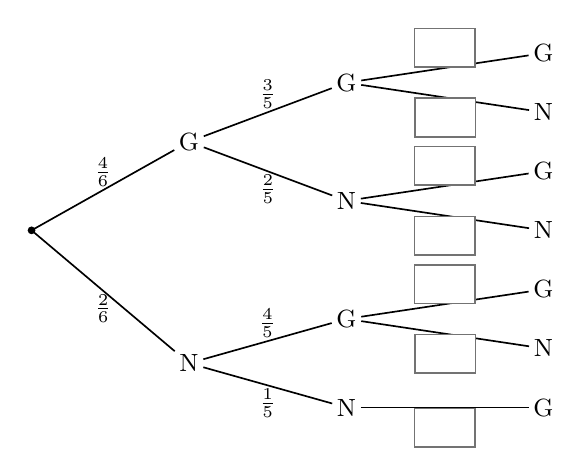
\begin{tikzpicture}[ak/.style={font=\small,inner sep=1.5pt,fill=white},wk/.style={font=\footnotesize,inner sep=1pt}]\fill (0,0) circle (1.4pt);\coordinate (s) at (0,0);\node[ak] (nG) at (2.00,1.125) {G};\node[ak] (nGG) at (4.00,1.875) {G};\node[ak] (nGGG) at (6.50,2.250) {G};\node[ak] (nGGN) at (6.50,1.500) {N};\node[ak] (nGN) at (4.00,0.375) {N};\node[ak] (nGNG) at (6.50,0.750) {G};\node[ak] (nGNN) at (6.50,0.000) {N};\node[ak] (nN) at (2.00,-1.688) {N};\node[ak] (nNG) at (4.00,-1.125) {G};\node[ak] (nNGG) at (6.50,-0.750) {G};\node[ak] (nNGN) at (6.50,-1.500) {N};\node[ak] (nNN) at (4.00,-2.250) {N};\node[ak] (nNNG) at (6.50,-2.250) {G};\draw[line width=0.6pt] (s) -- (nG) node[wk,above,pos=0.5] {$\frac{4}{6}$};\draw[line width=0.6pt] (nG) -- (nGG) node[wk,above,pos=0.5] {$\frac{3}{5}$};\draw[line width=0.6pt] (nGG) -- (nGGG) node[wk,above,draw=black!55,fill=white,pos=0.5] {\rule{0pt}{4.2mm}\rule{7mm}{0pt}};\draw[line width=0.6pt] (nGG) -- (nGGN) node[wk,below,draw=black!55,fill=white,pos=0.5] {\rule{0pt}{4.2mm}\rule{7mm}{0pt}};\draw[line width=0.6pt] (nG) -- (nGN) node[wk,below,pos=0.5] {$\frac{2}{5}$};\draw[line width=0.6pt] (nGN) -- (nGNG) node[wk,above,draw=black!55,fill=white,pos=0.5] {\rule{0pt}{4.2mm}\rule{7mm}{0pt}};\draw[line width=0.6pt] (nGN) -- (nGNN) node[wk,below,draw=black!55,fill=white,pos=0.5] {\rule{0pt}{4.2mm}\rule{7mm}{0pt}};\draw[line width=0.6pt] (s) -- (nN) node[wk,below,pos=0.5] {$\frac{2}{6}$};\draw[line width=0.6pt] (nN) -- (nNG) node[wk,above,pos=0.5] {$\frac{4}{5}$};\draw[line width=0.6pt] (nNG) -- (nNGG) node[wk,above,draw=black!55,fill=white,pos=0.5] {\rule{0pt}{4.2mm}\rule{7mm}{0pt}};\draw[line width=0.6pt] (nNG) -- (nNGN) node[wk,below,draw=black!55,fill=white,pos=0.5] {\rule{0pt}{4.2mm}\rule{7mm}{0pt}};\draw[line width=0.6pt] (nN) -- (nNN) node[wk,below,pos=0.5] {$\frac{1}{5}$};\draw[line width=0.6pt] (nNN) -- (nNNG) node[wk,below,draw=black!55,fill=white,pos=0.5] {\rule{0pt}{4.2mm}\rule{7mm}{0pt}};\end{tikzpicture}}{}{}
\medskip
\aufg{\hangindent7mm\hangafter1\nr{3.}Für einen Staffellauf wird die Reihenfolge von 8 Kindern ausgelost; jedes läuft genau einmal. Wie groß ist die Wahrscheinlichkeit, dass Nora unter den ersten drei Läufern ist? Sorten: Nora (1) und andere (7). Gib sie auch in Prozent an.}{}{}
\medskip
\aufg{\hangindent7mm\hangafter1\nr{4.}In einer Dose liegen 15 Bonbons: 8 blaue, 4 gelbe und 3 rote. Ben nimmt blind drei. Er sagt: „Es gibt doppelt so viele blaue wie gelbe. Also ist dreimal Blau doppelt so wahrscheinlich wie dreimal Gelb.“ Stimmt das? Wievielmal so wahrscheinlich ist dreimal Blau?}{}{{\scriptsize\color{mbgrau}Ziel\hspace{2mm}}}
\medskip
\par\vspace{3mm}\setlength{\kr}{\dimexpr\pagegoal-\pagetotal-10mm\relax}%
\ifdim\kr>12mm\karomerk{k}{C}\noindent{\scriptsize\color{mbgrau}Platz zum Rechnen}\par\nointerlineskip\vspace{1mm}\noindent
\begin{tikzpicture}\clip (0,0) rectangle ({\linewidth-0.5mm},\kr);\draw[black!16,line width=0.3pt,step=5mm] (0,0) grid (\linewidth,\kr);\end{tikzpicture}\fi\par
\clearpage\label{s:D}\noindent\colorbox{black!12}{\makebox[10mm]{\Large\bfseries\strut D}}\hspace{3mm}{\Large\bfseries Mit oder ohne Zurücklegen?}\par\smallskip
\noindent Kommt das Gezogene zurück (Zettel in den Topf, Glücksrad, Würfel), bleiben die Äste auf jeder Stufe gleich. Wird es behalten oder gegessen, ändern sie sich. Lies im Text, was mit dem ersten Stück passiert.\par\medskip
\noindent\textbf{Formel}\par\nopagebreak\noindent\hspace*{4mm}\begin{minipage}{\dimexpr\linewidth-4mm\relax}mit: $\dfrac{\text{rote}}{\text{alle}} \cdot \dfrac{\text{rote}}{\text{alle}}$ \qquad ohne: $\dfrac{\text{rote}}{\text{alle}} \cdot \dfrac{\text{rote} - 1}{\text{alle} - 1}$\end{minipage}\par\medskip
\noindent\textbf{Beispiel}\quad In einem Beutel liegen 3 rote und 2 blaue Kugeln. Zweimal wird eine Kugel gezogen. Vergleiche die Wahrscheinlichkeit für zweimal Rot mit und ohne Zurücklegen.\par\smallskip
\noindent\par\noindent\hangindent6mm\hangafter1\makebox[6mm][l]{\textbf{1}}Mit Zurücklegen: Die Kugel kommt zurück, beide Male 3 rote von 5: $\frac{3}{5} \cdot \frac{3}{5} = \frac{9}{25} = 36\,\%$.\par\smallskip\par\noindent\hangindent6mm\hangafter1\makebox[6mm][l]{\textbf{2}}Ohne Zurücklegen: beim 2. Zug nur noch 2 rote von 4: $\frac{3}{5} \cdot \frac{2}{4} = \frac{3}{10} = 30\,\%$.\par\smallskip\par\noindent\hangindent6mm\hangafter1\makebox[6mm][l]{\textbf{3}}Ohne Zurücklegen ist zweimal Rot seltener, um $36\,\% - 30\,\% = 6$ Prozentpunkte.\par\smallskip\par\medskip
\noindent\textbf{Aufgaben}\hspace{1em}{\small\color{mbgrau}\karohinweis{D}{Rechne unten im Karo.}{Rechne auf einem extra Blatt.} Vergleiche jede Aufgabe gleich mit dem Lösungsheft.}\par\smallskip
\aufg{\hangindent7mm\hangafter1\nr{1.}Bei welchem Versuch ändern sich die Äste der 2. Stufe? (Das ist Ziehen ohne Zurücklegen.) Kreuze an.\par\smallskip\leftskip7mm \kreuzl{Ein Würfel wird zweimal geworfen.}\kreuzl{Ein Glücksrad wird zweimal gedreht.}\kreuzl{Aus einer Tüte werden nacheinander zwei Gummibärchen gegessen.}\kreuzl{Ein Los wird gezogen, notiert und zurückgelegt; dann wird wieder gezogen.}}{}{}
\medskip
\aufg{\hangindent7mm\hangafter1\nr{2.}In einem Hut liegen 6 Zettel, auf 2 davon steht „Pause“. Es wird zweimal ein Zettel gezogen. Wie groß ist die Wahrscheinlichkeit für zweimal „Pause“, a) wenn der erste Zettel zurückgelegt wird, b) wenn er draußen bleibt?}{}{}
\medskip
\aufg{\hangindent7mm\hangafter1\nr{3.}Jeden Montag lost Frau Kaya aus einer Dose mit 5 Namenskärtchen ein Kind für den Tafeldienst aus. Danach steckt sie das Kärtchen wieder in die Dose. Wie groß ist die Wahrscheinlichkeit, dass Lina zwei Wochen hintereinander dran ist?}{}{}
\medskip
\aufg{\hangindent7mm\hangafter1\nr{4.}Sophie dreht zweimal ein Glücksrad mit 6 gleich großen Feldern, 3 davon rot. Marc zieht aus einem Beutel mit 6 Kugeln, 3 davon rot, zwei Kugeln ohne Zurücklegen. Wer hat die größere Wahrscheinlichkeit für zweimal Rot? Um wie viele Prozentpunkte?}{}{{\scriptsize\color{mbgrau}Ziel\hspace{2mm}}}
\medskip
\par\vspace{3mm}\setlength{\kr}{\dimexpr\pagegoal-\pagetotal-10mm\relax}%
\ifdim\kr>12mm\karomerk{k}{D}\noindent{\scriptsize\color{mbgrau}Platz zum Rechnen}\par\nointerlineskip\vspace{1mm}\noindent
\begin{tikzpicture}\clip (0,0) rectangle ({\linewidth-0.5mm},\kr);\draw[black!16,line width=0.3pt,step=5mm] (0,0) grid (\linewidth,\kr);\end{tikzpicture}\fi\par
\clearpage\label{s:T}\noindent\colorbox{black!12}{\makebox[10mm]{\Large\bfseries\strut T}}\hspace{3mm}{\Large\bfseries Probetest}\par\smallskip
\noindent Gemischt wie in der Prüfung, ohne Beispiel. Taschenrechner erlaubt. Etwa 20 Minuten.\par\medskip
\noindent\textbf{Aufgaben}\hspace{1em}{\small\color{mbgrau}\karohinweis{T}{Rechne unten im Karo.}{Rechne auf einem extra Blatt.} Vergleiche jede Aufgabe gleich mit dem Lösungsheft.}\par\smallskip
\aufgg{\hangindent7mm\hangafter1\nr{1.}In einer Kiste liegen 7 Äpfel, 2 davon sind faul (F), die anderen gut (G). Ben nimmt blind zwei. Ergänze die leeren Felder im Baum. Wie groß ist die Wahrscheinlichkeit, dass beide gut sind?}{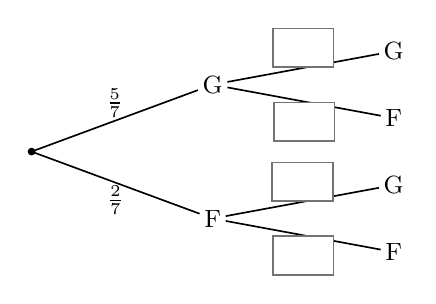
\begin{tikzpicture}[ak/.style={font=\small,inner sep=1.5pt,fill=white},wk/.style={font=\footnotesize,inner sep=1pt}]\fill (0,0) circle (1.4pt);\coordinate (s) at (0,0);\node[ak] (nG) at (2.30,0.850) {G};\node[ak] (nGG) at (4.60,1.275) {G};\node[ak] (nGF) at (4.60,0.425) {F};\node[ak] (nF) at (2.30,-0.850) {F};\node[ak] (nFG) at (4.60,-0.425) {G};\node[ak] (nFF) at (4.60,-1.275) {F};\draw[line width=0.6pt] (s) -- (nG) node[wk,above,pos=0.5] {$\frac{5}{7}$};\draw[line width=0.6pt] (nG) -- (nGG) node[wk,above,draw=black!55,fill=white,pos=0.5] {\rule{0pt}{4.2mm}\rule{7mm}{0pt}};\draw[line width=0.6pt] (nG) -- (nGF) node[wk,below,draw=black!55,fill=white,pos=0.5] {\rule{0pt}{4.2mm}\rule{7mm}{0pt}};\draw[line width=0.6pt] (s) -- (nF) node[wk,below,pos=0.5] {$\frac{2}{7}$};\draw[line width=0.6pt] (nF) -- (nFG) node[wk,above,draw=black!55,fill=white,pos=0.5] {\rule{0pt}{4.2mm}\rule{7mm}{0pt}};\draw[line width=0.6pt] (nF) -- (nFF) node[wk,below,draw=black!55,fill=white,pos=0.5] {\rule{0pt}{4.2mm}\rule{7mm}{0pt}};\end{tikzpicture}}{}{}
\medskip
\aufg{\hangindent7mm\hangafter1\nr{2.}In einem Glas sind 3 Kirsch- und 3 Zitronenbonbons. Ina nimmt blind zwei. Wie groß ist die Wahrscheinlichkeit für zwei gleiche Sorten? Kreuze an.\par\medskip\noindent\hspace*{7mm}\mbox{$\square$\ $\dfrac{1}{4}$}\hspace{10mm}\mbox{$\square$\ $\dfrac{2}{5}$}\hspace{10mm}\mbox{$\square$\ $\dfrac{1}{2}$}\hspace{10mm}\mbox{$\square$\ $\dfrac{3}{5}$}\rule[-3mm]{0pt}{8mm}\par\smallskip }{}{}
\medskip
\aufg{\hangindent7mm\hangafter1\nr{3.}Im Lostopf der Klasse liegen 25 Zettel mit allen Namen. Jede Woche wird ein Zettel gezogen, wer ihn hat, macht den Wochendienst; danach kommt der Zettel zurück. Wie groß ist die Wahrscheinlichkeit, dass Tim zwei Wochen hintereinander dran ist? Gib sie auch in Prozent an.}{}{}
\medskip
\aufg{\hangindent7mm\hangafter1\nr{4.}In einer Lostrommel sind 10 Lose, 3 davon gewinnen. Kai zieht nacheinander drei Lose. Wie groß ist die Wahrscheinlichkeit, dass mindestens ein Gewinn dabei ist? Gib sie in Prozent an (eine Stelle nach dem Komma).}{}{}
\medskip
\aufg{\hangindent7mm\hangafter1\nr{5.}Auf einem Blech liegen 12 Muffins, die gleich aussehen: 9 mit Schokolade (S), 3 mit Kirsche (K). Jan nimmt nacheinander zwei. a) Schreibe alle Ergebnisse auf, bei denen mindestens ein Kirschmuffin dabei ist. b) Berechne die Wahrscheinlichkeit, dass beide mit Schokolade sind. c) Jan sagt: „Mindestens einen Kirschmuffin zu erwischen ist wahrscheinlicher als zwei mit Schokolade.“ Hat er recht?}{}{{\scriptsize\color{mbgrau}Ziel\hspace{2mm}}}
\medskip
\par\vspace{3mm}\setlength{\kr}{\dimexpr\pagegoal-\pagetotal-10mm\relax}%
\ifdim\kr>12mm\karomerk{k}{T}\noindent{\scriptsize\color{mbgrau}Platz zum Rechnen}\par\nointerlineskip\vspace{1mm}\noindent
\begin{tikzpicture}\clip (0,0) rectangle ({\linewidth-0.5mm},\kr);\draw[black!16,line width=0.3pt,step=5mm] (0,0) grid (\linewidth,\kr);\end{tikzpicture}\fi\par
\end{document}
